\documentclass[14pt]{article}
\title{Lab2 Report}
\author{Zepeng Chen}
\date{\today}
\usepackage{listings}
\usepackage{color}
\usepackage{graphicx}
\usepackage{subcaption}
\usepackage{gensymb}
\usepackage{geometry}
\geometry{a4paper,left=2cm,right=2cm,top=1cm,bottom=1cm}

\definecolor{dkgreen}{rgb}{0,0.6,0}
\definecolor{gray}{rgb}{0.5,0.5,0.5}
\definecolor{mauve}{rgb}{0.58,0,0.82}

\lstset{frame=tb,
	language=Python,
	aboveskip=3mm,
	belowskip=3mm,
	showstringspaces=false,
	columns=flexible,
	basicstyle={\small\ttfamily},
	numbers=none,
	numberstyle=\tiny\color{gray},
	keywordstyle=\color{blue},
	commentstyle=\color{dkgreen},
	stringstyle=\color{mauve},
	breaklines=true,
	breakatwhitespace=true,
	tabsize=3
}

\begin{document}
	\maketitle
	\tableofcontents
	\section{Spatial Filtering}
	\subsection{Implemented Function}
	\lstinputlisting[breaklines]{lab2.py}
	\newcommand{\RNum}[1]{\uppercase\expandafter{\romannumeral #1\relax}}
	\subsection{Outcome Collection \RNum{1}}
	\newpage
	\begin{figure}[hbt!]
		\centering
		\begin{subfigure}[b]{0.23\linewidth}
			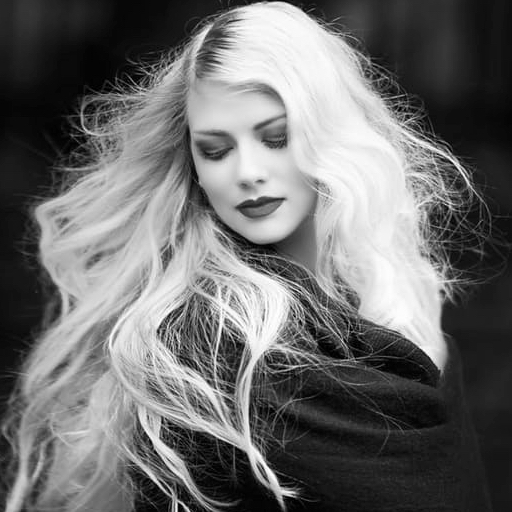
\includegraphics[width=\linewidth]{origin.png}
			\caption{Original Image.}
		\end{subfigure}
		\begin{subfigure}[b]{0.23\linewidth}
			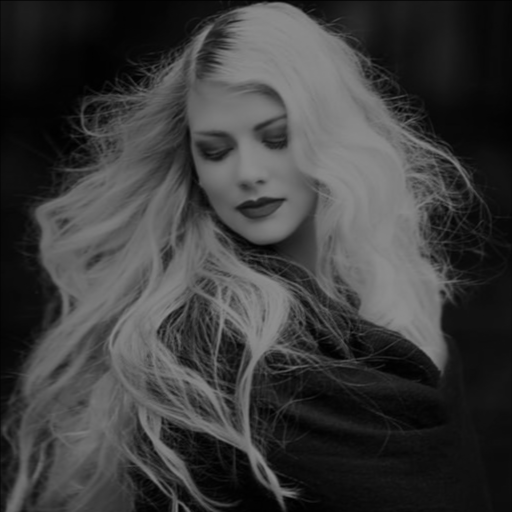
\includegraphics[width=\linewidth]{ones3.png}
			\caption{Ones(3)}
		\end{subfigure}
		\begin{subfigure}[b]{0.23\linewidth}
			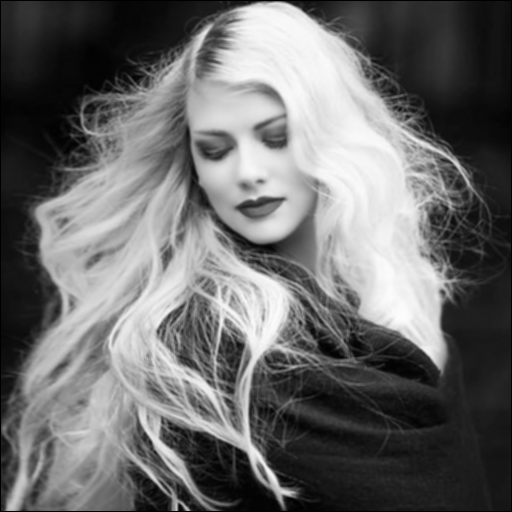
\includegraphics[width=\linewidth]{ones7.png}
			\caption{ones(7)}
		\end{subfigure}
		\begin{subfigure}[b]{0.23\linewidth}
			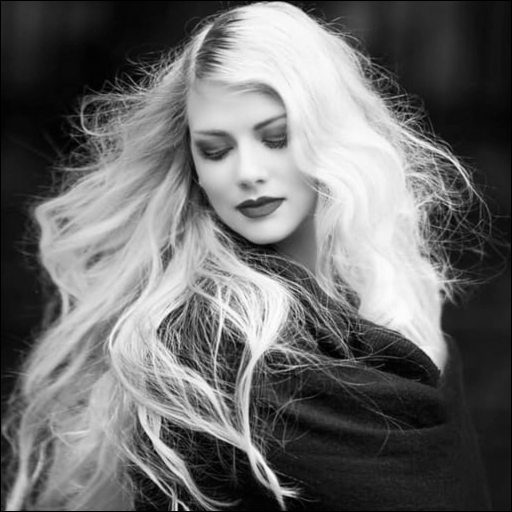
\includegraphics[width=\linewidth]{g3.png}
			\caption{Gaussian3}
		\end{subfigure}
		\begin{subfigure}[b]{0.23\linewidth}
			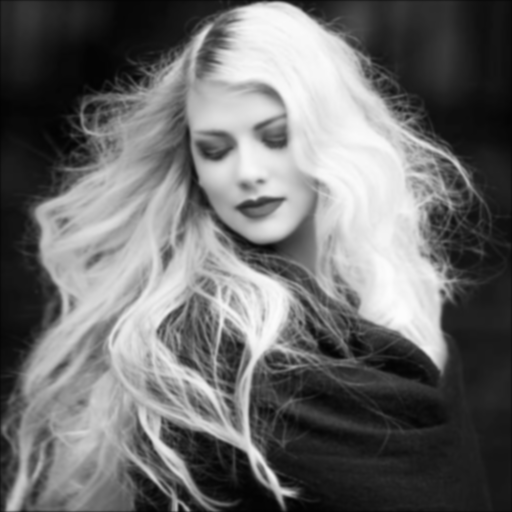
\includegraphics[width=\linewidth]{g7.png}
			\caption{Gaussian7}
		\end{subfigure}
		\begin{subfigure}[b]{0.23\linewidth}
			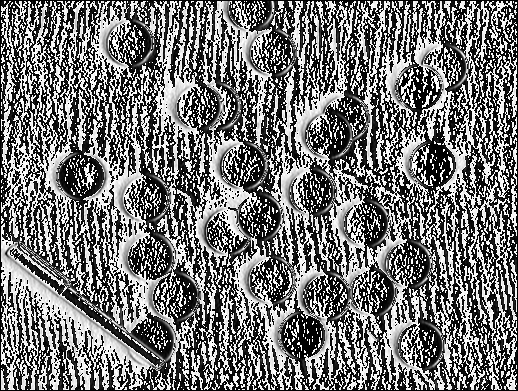
\includegraphics[width=\linewidth]{k6.png}
			\caption{Sobel-x}
		\end{subfigure}
		\begin{subfigure}[b]{0.23\linewidth}
			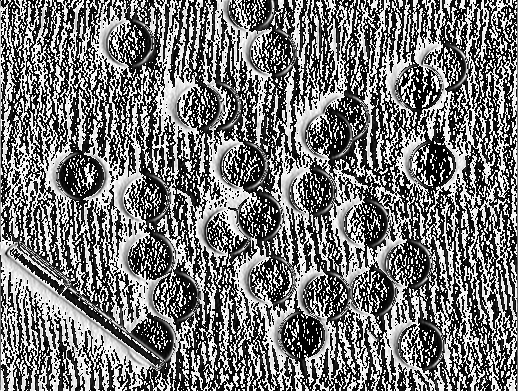
\includegraphics[width=\linewidth]{k7.png}
			\caption{Sobel-y}
		\end{subfigure}
		\begin{subfigure}[b]{0.23\linewidth}
			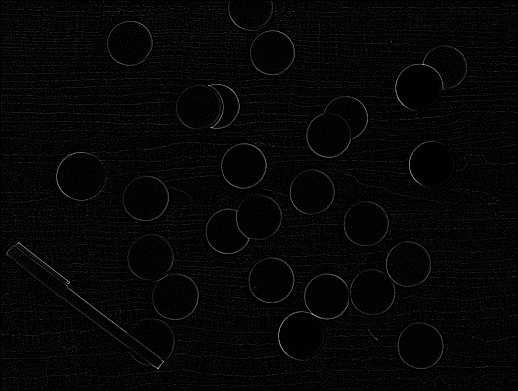
\includegraphics[width=\linewidth]{log3.png}
			\caption{log3}
		\end{subfigure}
	\end{figure}
	\section{Median Filter}
	\subsection{Code}
	\lstinputlisting[breaklines]{med.py}
	\subsection{Figure Collection \RNum{2}}
	\newpage
	\begin{figure}[hbt!]
		\centering
	\begin{subfigure}[b]{0.4\linewidth}
		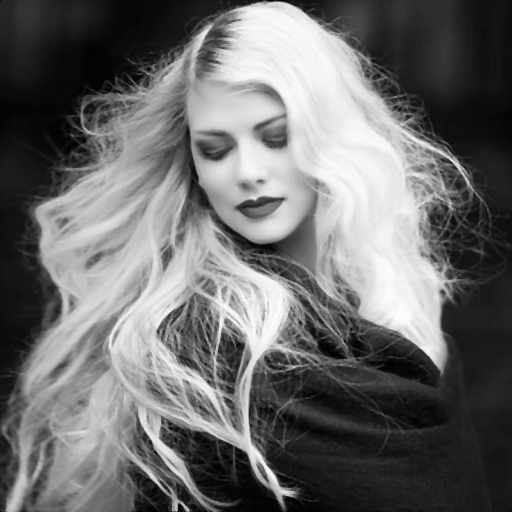
\includegraphics[width=\linewidth]{m3.png}
		\caption{Median3X3}
	\end{subfigure}
	\begin{subfigure}[b]{0.4\linewidth}
		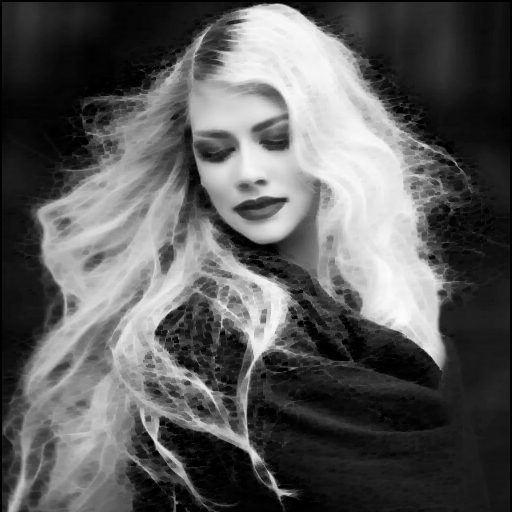
\includegraphics[width=\linewidth]{m5.png}
		\caption{Median5X5}
	\end{subfigure}
	\end{figure}
\section{Thresholding}
\subsection{Code for fingding threshold}
\lstinputlisting[breaklines]{thresholding.py}
\end{document}